\documentclass{article}
\usepackage{amssymb}
\usepackage{amsmath}
\usepackage{tikz}

\begin{document}

  \section{Punto 1}
    Considere el anillo $\mathbb{Z}[i]$. Asuma que las unidades de $\mathbb{Z}[i]$ son 
    $\pm 1$ y $\pm i$.

    \subsection{Subpunto a)}
      Sea $\pi \in \mathbb{Z}[i]$ un elemento primo. Demuestre que $\pi$ y $\overline{\pi}$ 
      son asociados si y solo si $\pi$ es asociado a un entero primo o $\pi \overline{\pi} = 2$.


      Empecemos asumiendo que $\pi$ y $\overline{\pi}$ son asociados, es decir, que si $\pi = a + b i$, entonces 
      \[a + b i = u \cdot (a - bi)\text{ con } u \in \{\pm 1, \pm i\}\]

      Analicemos cada posible valor de $u$: 

      \begin{itemize}

        \item Cuando $u = 1$: $a + bi = a - bi$, luego $b = 0$, entonces $a$ es primo en $\mathbb{Z}$,
          luego, $\pi$ es asociado a un entero primo.

        \item Cuando $u = -1$: $a + bi = -a + bi$, entonces $a = 0$ y por el mismo razonamiento anterior, 
              $b$ es primo por ser $\pi$ primo y son asociados ($b = -i \pi$).

        \item Cuando $u = i$: $a + bi = i(a - bi) = ia + b$, entonces $b = a$, luego $\pi = a(1 + i)$. 
              Como $\pi$ es primo y $1 + i$ no es una unidad, entonces $a$ lo es, luego 

              \[
                a(1 + i) a (1 - i) = a^2 (1 - i + i + 1) = 2
              \]

        \item Si $u = -i$: $a + bi = -i(a - bi) = -ia - b$, luego $b = -a$, resultando en que 
              $\pi = a(1 - i)$ y como $\pi$ es primo, entonces $a$ es unidad, resultado en el mismo 
              razonamiento que en el item anterior.
      \end{itemize}

      con esto concluimos lo solicitado por la primera implicación.

      Ahora vamos a sumir que $\pi$ es asocidado a un primo o $\pi \overline{pi} = 2$.

      \begin{itemize}
        \item Si $\pi$ es asociado a un primo entero, entonces $\pi = u p$, luego $\overline{\pi} = \overline{u} p$, 
              si $u$ no es entero, entonces $\pi = -\overline{\pi}$, si $u = \pm i$ y $\pi = \overline{\pi}$ 
              si $u = \pm 1$

            \item  Si $\pi \overline{\pi} = 2$, entonces $a^2 + b^2 = 2$, entonces $a, b \in \{\pm 1\}$, se verifican
                   para los 4 casos:

                   \begin{equation*}
                     \begin{aligned}
                       (\pi = 1 + i & \iff & \overline{\pi} = 1 - i) & \Rightarrow &  i\overline{\pi} = \pi \\
                       (\pi = -1 + i & \iff & \overline{\pi} = -1 - i) & \Rightarrow &  -i\overline{\pi} = \pi \\
                     \end{aligned}
                   \end{equation*}
      \end{itemize}

    \subsection{Subpunto b)}
      Sea $p \in \mathbb{Z}$ un primo. Demuestre que $p$ es primo en $\mathbb{Z}[i]$ o 
      $p = \pi \overline{\pi}$ con $\pi$ primo en $\mathbb{Z}[i]$.

      Si $p$ no se puede reducir, entonces sería primo en $\mathbb{Z}[i]$ por ser este un anillo euclidiano.


      Si por el contrario, $p = ab$ sin ser unidad alguno de ellos, entonces 
      \[
        N(p) = N(a)N(b) \Rightarrow p^2 = N(a)N(b)
      \]

      Pero como $N(a), N(b) > 1$ (por no ser unidades), entonces $N(a) = p = N(b)$, luego 
      $p = N(a)$, pero la norma de $\mathbb{Z}[i]$ es $a \overline{a}$, entonces 
      \[
        p = a \overline{a}
      \]

  \pagebreak
  \section{punto 2} 
  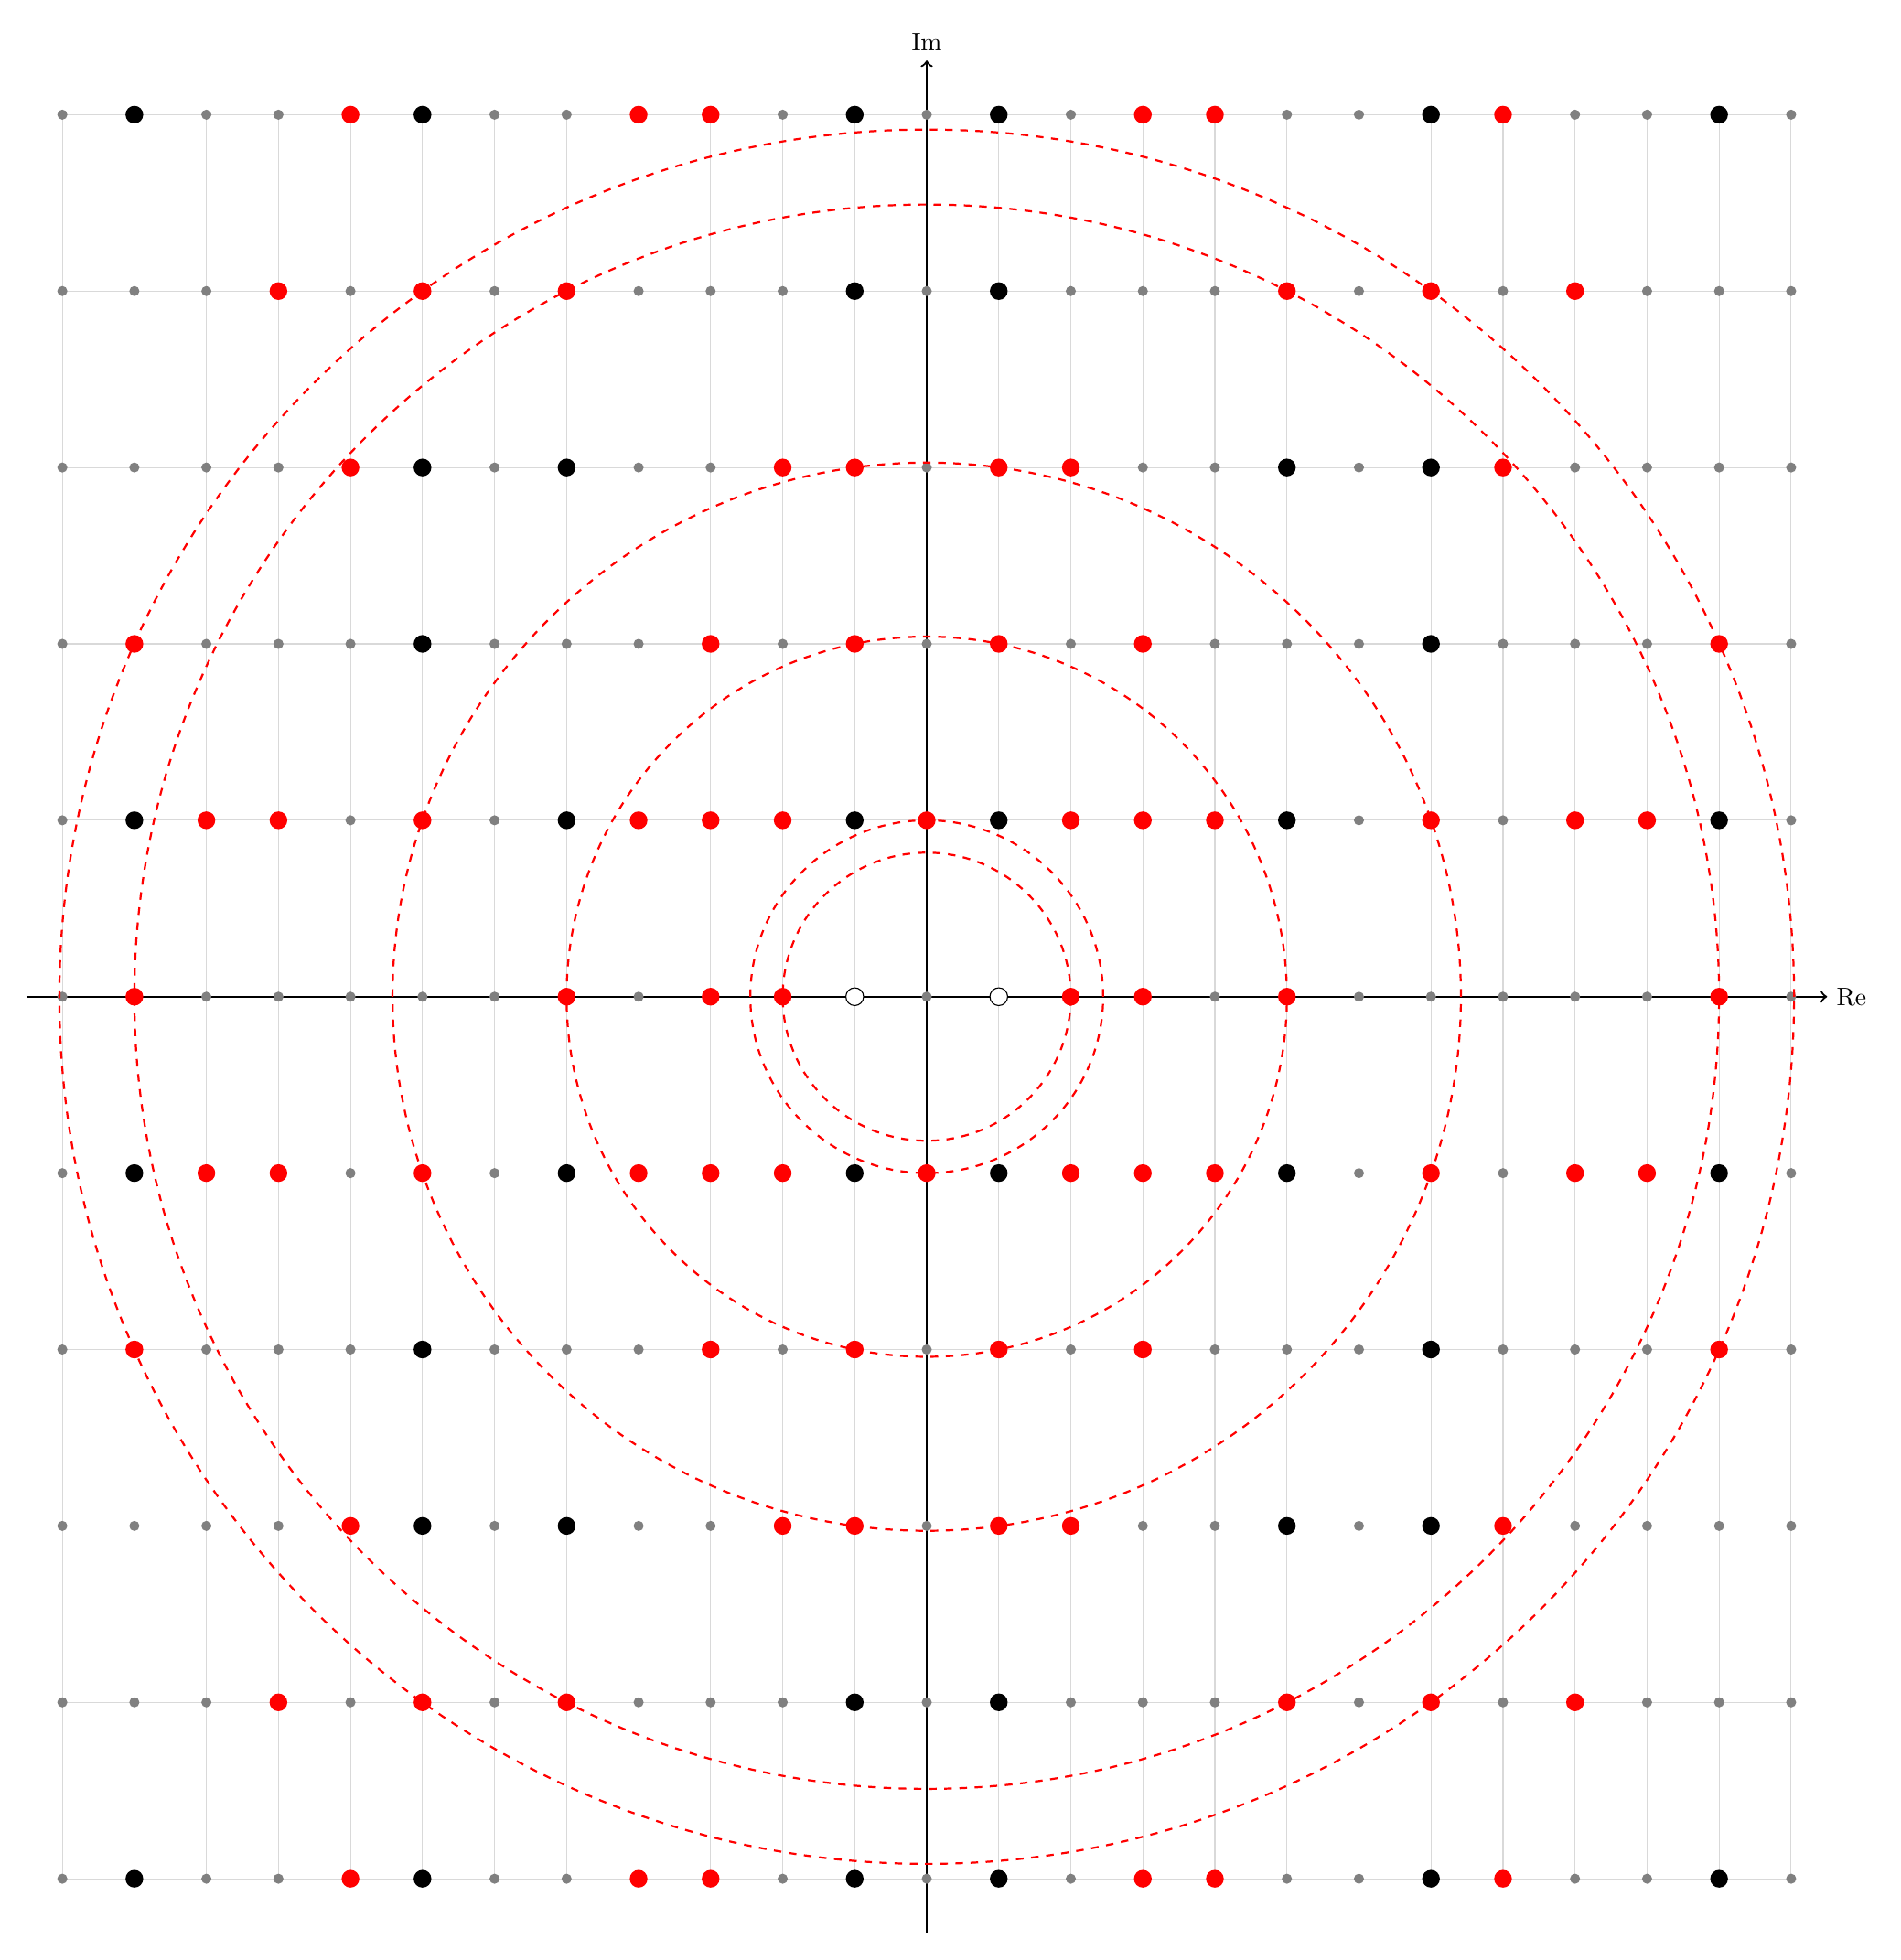
\begin{tikzpicture}[scale=1]
    
    \def\sqrtsix{2.44949}

    
    \foreach \a in {-12,...,12} {
        \draw[gray!30, thin] (\a, -5*\sqrtsix) -- (\a, 5*\sqrtsix);
    }
    \foreach \b in {-5,...,5} {
        \draw[gray!30, thin] (-12, \b*\sqrtsix) -- (12, \b*\sqrtsix);
    }
    \draw[->, thick] (-12.5, 0) -- (12.5, 0) node[right] {Re};
    \draw[->, thick] (0, -13) -- (0, 13) node[above] {Im};

    
    \foreach \a in {-12,...,12} {
        \foreach \b in {-5,...,5} {
            \fill[gray] (\a, \b*\sqrtsix) circle (2pt);
        }
    }

    
    \foreach \a/\b in {1/0, -1/0} {
        \fill[white] (\a, \b*\sqrtsix) circle (3.5pt);
        \draw[black] (\a, \b*\sqrtsix) circle (3.5pt);
    }


    \foreach \a/\b in {2/0, -2/0, 0/1, 0/-1} { 
        \fill[red] (\a, \b*\sqrtsix) circle (3.5pt);
    } 
    \draw[thick, red, dashed] (0,0) circle (2cm);
    \draw[thick, red, dashed] (0,0) circle (2.449cm);
    
    \foreach \a/\b in {5/0, -5/0, 1/2, -1/2, 1/-2, -1/-2} { 
        \fill[red] (\a, \b*\sqrtsix) circle (3.5pt);
    }
    \draw[thick, red, dashed] (0,0) circle (5cm);
    
   
    \foreach \a/\b in {11/0, -11/0, 5/4, -5/4, 5/-4, -5/-4} {
        \fill[red] (\a, \b*\sqrtsix) circle (3.5pt);
    }
    \draw[thick, red, dashed] (0,0) circle (11cm);

    
    \draw[thick, red, dashed] (0,0) circle (7.416cm);
    
    \draw[thick, red, dashed] (0,0) circle (12.041cm);

    
    \foreach \a/\b in {
        3/0, -3/0,                                     
        2/1, -2/1, 2/-1, -2/-1,                        
        3/1, -3/1, 3/-1, -3/-1,                        
        4/1, -4/1, 4/-1, -4/-1,                        
        7/1, -7/1, 7/-1, -7/-1,                        
        1/3, -1/3, 1/-3, -1/-3,                        
        9/1, -9/1, 9/-1, -9/-1,                        
        10/1, -10/1, 10/-1, -10/-1,                    
        3/2, -3/2, 3/-2, -3/-2,                        
        11/2, -11/2, 11/-2, -11/-2,                    
        7/4, -7/4, 7/-4, -7/-4,                        
        2/3, -2/3, 2/-3, -2/-3,                        
        8/3, -8/3, 8/-3, -8/-3,                        
        9/4, -9/4, 9/-4, -9/-4,                        
        3/5, -3/5, 3/-5, -3/-5,                        
        4/5, -4/5, 4/-5, -4/-5,                        
        8/5, -8/5, 8/-5, -8/-5                         
    } {
        \fill[red] (\a, \b*\sqrtsix) circle (3.5pt);
    }
    
    \foreach \a/\b in {
        1/1, -1/1, 1/-1, -1/-1,                         
        5/1, -5/1, 5/-1, -5/-1,                        
        7/2, -7/2, 7/-2, -7/-2,                        
        5/3, -5/3, 5/-3, -5/-3,                        
        1/4, -1/4, 1/-4, -1/-4,                        
        7/3, -7/3, 7/-3, -7/-3,                        
        11/1, -11/1, 11/-1, -11/-1,                    
        1/5, -1/5, 1/-5, -1/-5,                        
        7/5, -7/5, 7/-5, -7/-5,                        
        11/5, -11/5, 11/-5, -11/-5                     
    } {
        \fill[black] (\a, \b*\sqrtsix) circle (3.5pt);
    }

\end{tikzpicture}
\pagebreak

  \section{Punto 3}

    \subsection{Subpunto a)}
      Con el procedimiento mostrado en la guía, divida $a = 9 + 8i$ entre $b = 3 + i$.


      A continuación se muestra el análisis geométrico:



      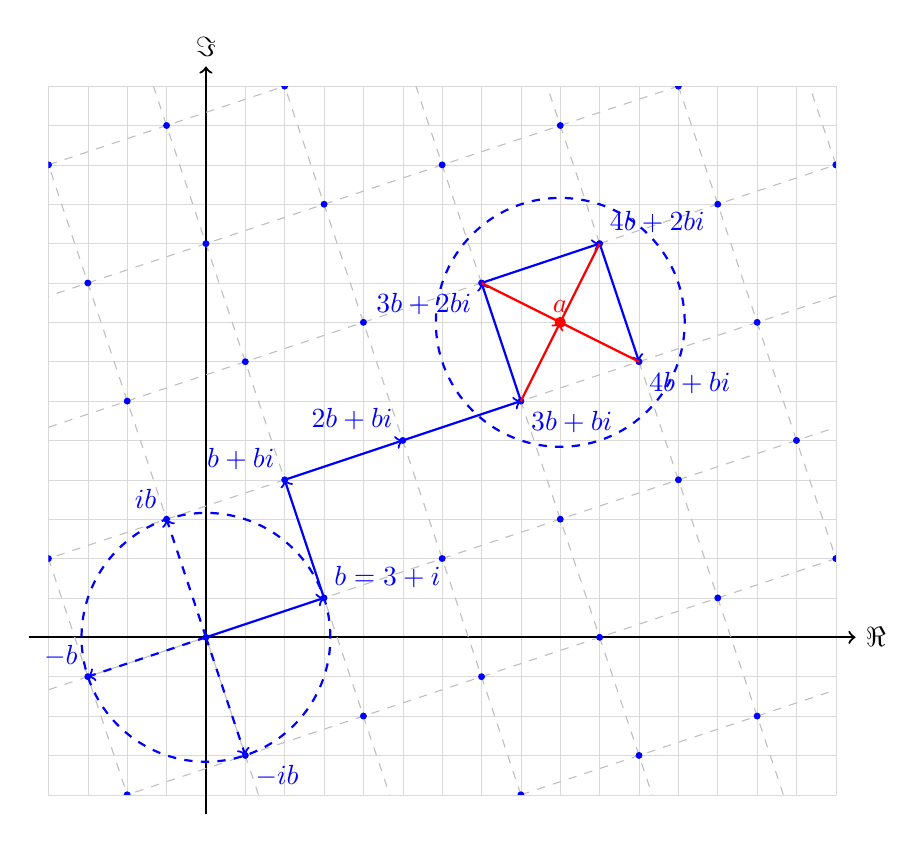
\begin{tikzpicture}[scale=0.5]
        \draw[gray!30, step=1, very thin] (-4,-4) grid (16,14);

        \draw[->, thick] (-4.5, 0) -- (16.5, 0) node[right] {$\Re$};
        \draw[->, thick] (0, -4.5) -- (0, 14.5) node[above] {$\Im$};

        \begin{scope}
          \clip (-4,-4) rectangle (16,14);

          \foreach \m in {-3,...,6} {
            \draw[gray!50, dashed, thin] ({- \m - 30}, {3*\m - 10}) -- ({- \m + 30}, {3*\m + 10});
          }

          \foreach \k in {-3,...,7} {
            \draw[gray!50, dashed, thin] ({3*\k + 10}, {\k - 30}) -- ({3*\k - 10}, {\k + 30});
          }

          \foreach \m in {-5,...,8} {
            \foreach \n in {-5,...,8} {
              \fill[blue] ({3*\m - \n}, {\m + 3*\n}) circle (2.5pt);
            }
          }
        \end{scope}

        \draw[blue, dashed, thick] (0, 0) circle (3.16);
        \draw[blue, dashed, thick] (9, 8) circle (3.16);

        \draw[->, thick, blue] (0, 0) -- (3, 1) node[above right] {$b = 3 + i$};
        \draw[->, thick, dashed, blue] (0, 0) -- (-1, 3) node[above left] {$ib$};
        \draw[->, thick, dashed, blue] (0, 0) -- (-3, -1) node[above left] {$-b$};
        \draw[->, thick, dashed, blue] (0, 0) -- (1, -3) node[below right] {$-ib$};

        \fill[red] (9, 8) circle (4pt) node[above, text=red] {$a$};

        \draw[->, thick, blue] (3, 1) -- (2, 4) node[above left] {$b + bi$};
        \draw[->, thick, blue] (2, 4) -- (5, 5) node[above left] {$2b + bi$};
        \draw[->, thick, blue] (5, 5) -- (8, 6) node[below right] {$3b + bi$};

        \draw[->, thick, blue] (8, 6) -- (7, 9) node[below left] {$3b + 2bi$};
        \draw[->, thick, blue] (7, 9) -- (10, 10) node[above right] {$4b + 2bi$};
        \draw[->, thick, blue] (10, 10) -- (11, 7) node[below right] {$4b + bi$};

        \draw[->, thick, red] (8, 6) -- (9, 8);
        \draw[-, thick, red] (7, 9) -- (9, 8);
        \draw[-, thick, red] (10, 10) -- (9, 8);
        \draw[-, thick, red] (11, 7) -- (9, 8);
      \end{tikzpicture}

      Vemos entonces lo siguiente:

      \begin{equation*}
        \begin{aligned}
          (3 + i)(3 + i) + 1 + 2i &= 9 + 3i + 3i - 1 + 1 + 2i &= 9 + 8i \\
          (3 + i)(3 + 2i) + 2 - i &= 9 + 6i + 3i - 2 + 2 - i  &= 9 + 8i \\
          (3 + i)(4 + 2i) -1 - 2i &= 12 + 6i + 4i - 2 - 1 -2i &= 9 + 8i \\
          (3 + i)(4 + i) -2 + i   &= 12 + 3i + 4i -1 - 2 + i  &= 9 + 8i
        \end{aligned}
      \end{equation*}

      La norma de $b$ es 10, la norma de cualquier residuo de lo vistos anteriormente es 5.

    \subsection{Subpunto b)}
      Generalice el resultado geométrico.


      La idea, es que siempre existen multiplos de $b$ dentro del circulo de rádio $|b|$, siendo $|\cdot|$ 
      la norma compleja.

      Si $a' = a + bi$, $b' = c + di$, sabemos que en la división de complejos, existen $x, y$ reales
      de tal modo que $\frac{a + bi}{c + di} = x + yi$. Como el cociente debe ser un entero de Gauss,
      escogemos $e, f$ enteros de tal modo que $|x - e| < \frac{1}{2}$ y $|y - f| < \frac{1}{2}$ (los
      enteros más cercanos en la recta real a cada número). 

      Si decimos que el cociente es $e + fi$ debemos verificar una condición importante, que este número 
      se encuentra dentro del círculo de centro $a'$ y de radio $|b|$, o de forma equivalente, que $N(a' - b'(e + fi)) < c^2 + d^2$.

      Sabemos que 

      \[
        (x - e)^2 + (y - f)^2 \leq \frac{1}{4} + \frac{1}{4} = \frac{1}{2}
      \]

      Luego, $N(\frac{a'}{b'} - (e + fi)) \leq \frac{1}{2}$, entonces $N(a' - b'(e + fi)) \leq \frac{1}{2}N(b') \leq N(b')$, 
      luego, $a' = b'(e + fi) + r$, donde $r = a' - b'(e + fi)$.

    \subsection{Subpunto c)}
      Usando un análisis geométrico similar al del taller, muestre que $\mathbb{Z}[\sqrt{-6}]$ no es 
      un anillo euclidiano.

      Para este ejemplo, tomamos $b = 5 + 2 \sqrt{-6}$ y el punto $a = 15$. Se puede ver 
      que no hay multiplos de $b$ dentro del circulo al rededor de $a$, por lo tanto no es posible 
      hacer la división, por no tener un residuo con menor norma.

      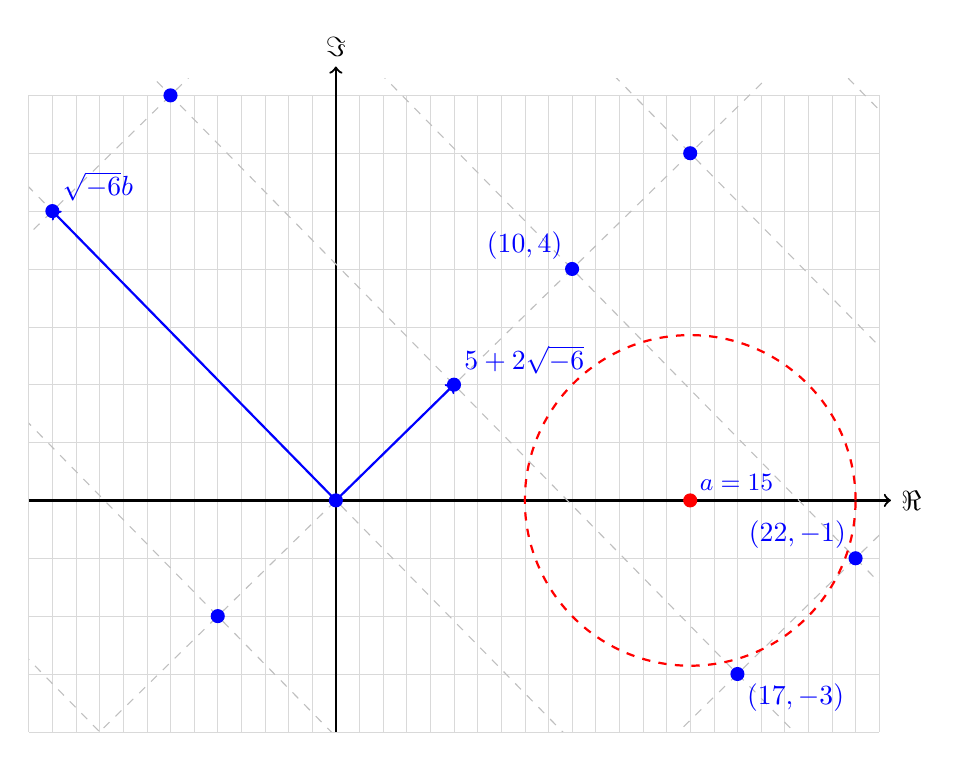
\begin{tikzpicture}[scale=0.3, yscale={sqrt(6)}]
        \draw[gray!30, step=1, very thin] (-13,-4) grid (23,7);
        \draw[->, thick] (-13, 0) -- (23.5, 0) node[right] {$\Re$};
        \draw[->, thick] (0, -4) -- (0, 7.5) node[above] {$\Im$};

        \begin{scope}
          \clip (-13,-4) rectangle (23, 7.3);

          \foreach \n in {-4,...,4} {
            \draw[gray!50, dashed, thin]
              ({-12*\n - 5*10}, {5*\n - 2*10}) -- ({-12*\n + 5*10}, {5*\n + 2*10});
          }

          \foreach \m in {-2,...,8} {
            \draw[gray!50, dashed, thin] 
              ({5*\m + 12*10}, {2*\m - 5*10}) -- ({5*\m - 12*10}, {2*\m + 5*10});
          }

          \foreach \m in {-1,...,5} {
            \foreach \n in {-2,...,2} {
              \node[circle, fill=blue, inner sep=1.8pt] at ({5*\m - 12*\n}, {5*\n + 2*\m}) {};
            }
          }

          \node[circle, fill=red, inner sep=1.8pt] at (15, 0) {};

          \node[blue, above right, font=\small] at (15, 0) {$a = 15$};

          \draw[red, dashed, thick] (15, 0) circle [x radius=7, y radius=2.857];

          \node[blue, below right] at (17, -3) {$(17,-3)$};
          \node[blue, above left] at (10, 4) {$(10,4)$};
          \node[blue, above left] at (22, -1) {$(22, -1)$};


          \draw[->, thick, blue] (0, 0) -- (5, 2) node[above right] {$5 + 2\sqrt{-6}$};
          \draw[->, thick, blue] (0, 0) -- (-12, 5) node[above right] {$\sqrt{-6}b$};
        \end{scope}
      \end{tikzpicture}
\end{document}
